\chapter{Experiments \label{cha:chapter4}}


\section{Dataset}


\subsection{MNIST}
MNIST\cite{LeCunMNISThandwrittendigit2010} is one of the most popular dataset that machine learning partitioners use to benchmark machine learning algorithms. The dataset consists of 60,000 training and 10,000 testing samples. Each sample is a grayscale 28x28 image of a digit between from 0 to 9. 

\begin{figure}[h]
\centering
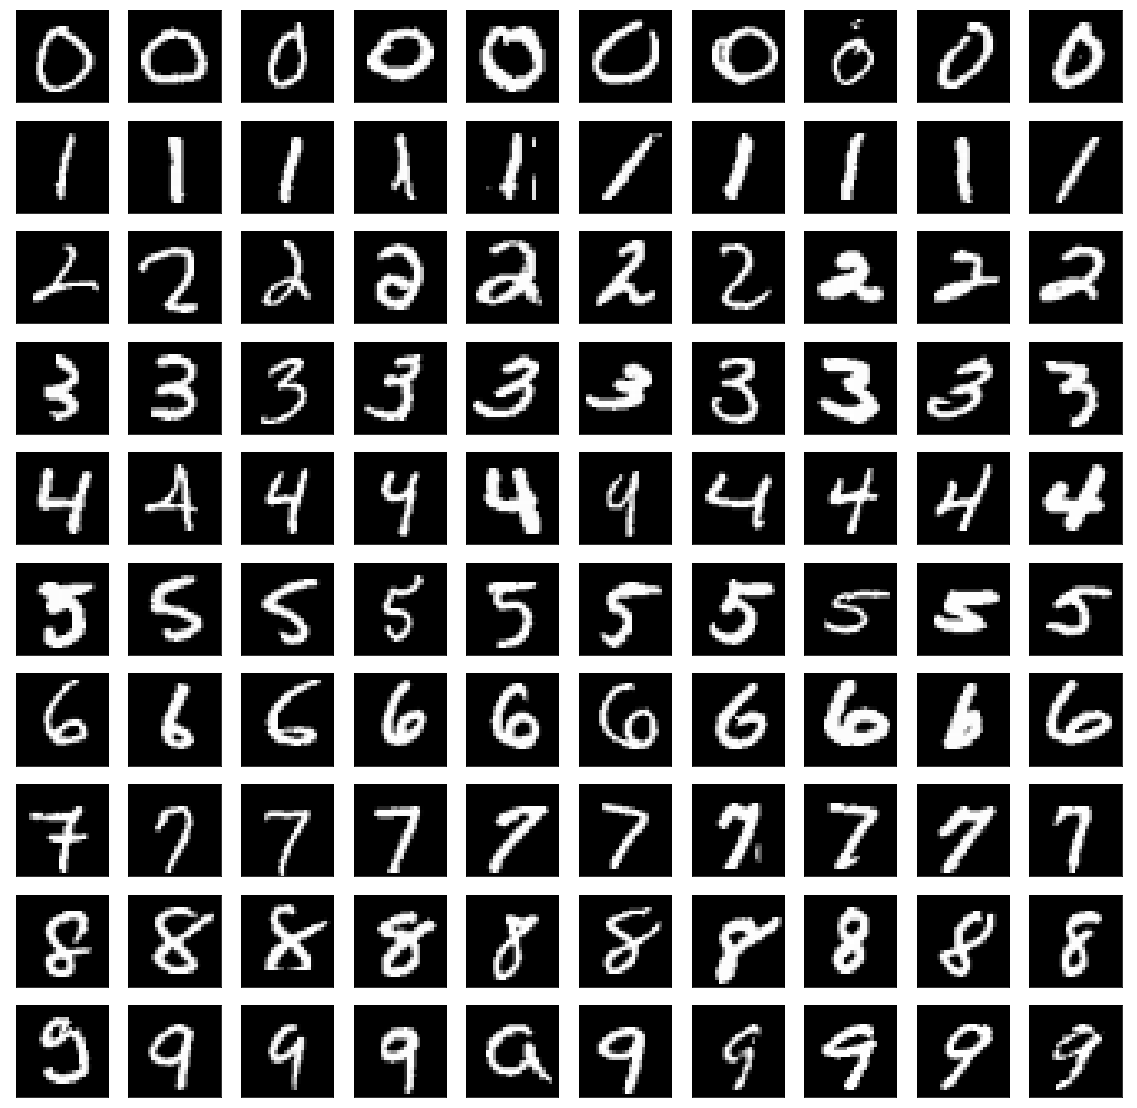
\includegraphics[width=0.5\textwidth]{mnist}
\caption{MNIST Dataset}
\label{fig:mnist_samples}
\end{figure}

State-of-the-art algorithms can classify MNIST with accuracy higher than 0.99, while classical ones, such as SVC or RandomForest, are able to achieve around 0.97\cite{XiaoFashionMNISTNovelImage2017}.


\subsection{Fashion-MNIST}

Xiao et. al.\cite{XiaoFashionMNISTNovelImage2017} propose a novel dataset, called Fashion-MNIST dataset, as a replacement of MNIST dataset for benchmarking machine learning algorithms.  According to \cite{XiaoFashionMNISTNovelImage2017},  Fashion-MNIST brings more challenging to the problem and more representative to modern computer vision tasks. It contains images of fashion products from 10 categories. Fashion-MNIST is comparable to MNIST in every aspects, such as the size of training and testing set, image dimension and data format, hence one can easily  apply existing algorithms that work with MNIST to Fashion-MNIST without any change.

\begin{figure}[h]
\centering
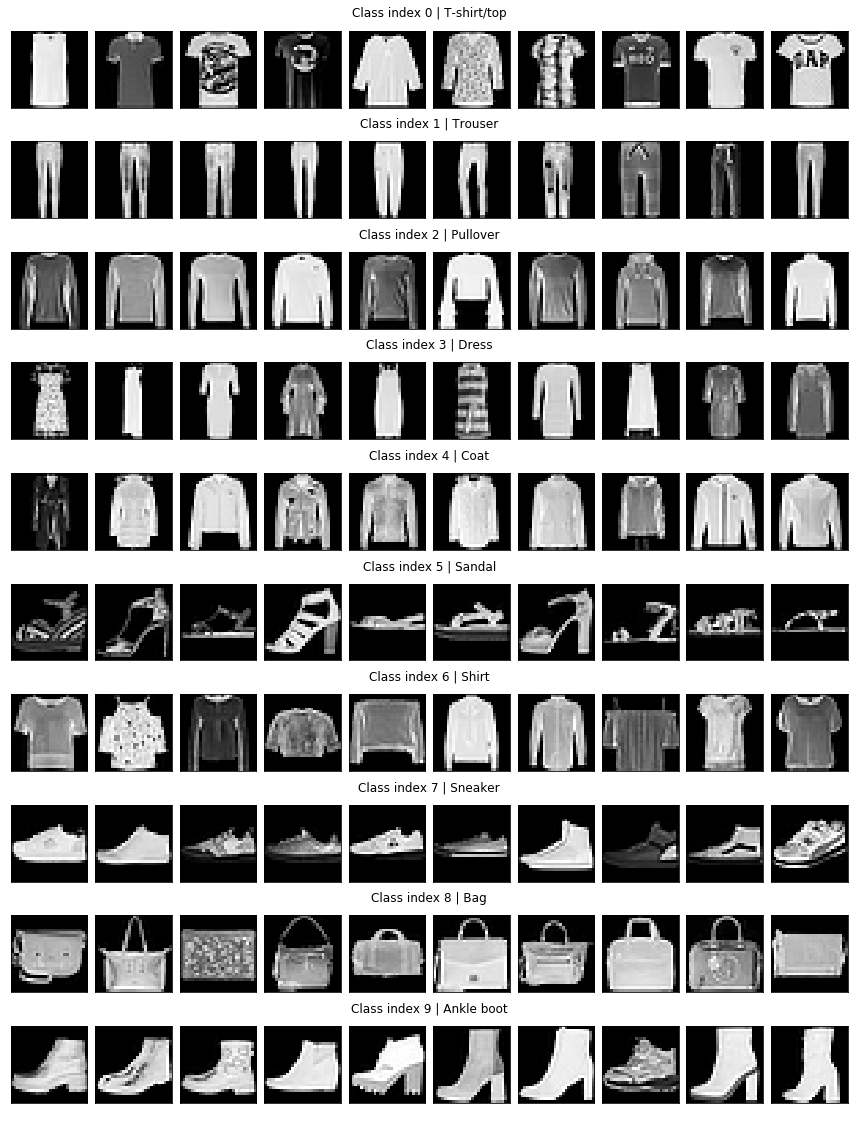
\includegraphics[width=0.6\textwidth]{fashion_mnist}
\caption{Fashion-MNIST Dataset\todo{use same size as MNIST figure}}
\label{fig:mnist_samples}
\end{figure}

\citep{XiaoFashionMNISTNovelImage2017} also reports benchmarking results of classical machine learning algorithms on Fashion-MNIST. On average, they achieve accuracy between 0.85 to 0.89. According to Fashion-MNIST's page\footnote{https://github.com/zalandoresearch/fashion-mnist}, A. Brock reports the state-of-the-art result  with 0.97 accuracy using Wide Residual Network(WRN)\cite{ZagoruykoWideResidualNetworks2016} and standard data preprocessing and augmentation.


\section{RNN Cell Architectures}
In this section, I will describe architectures or RNN cell evaluated in this thesis.  To make the descriptions concise, I denote notations as follows: 

\begin{itemize}
	\item $\patvector{a}_{t}^{(l)}$ : activation vector of layer $l$ at step $t$
	\item $\patvector{x}_t$ : subset of $x_i \in \patvector{x}$ corresponding to step $t$ and assume to be reshaped into a column vector
\end{itemize}

\subsection{Shallow Cell}
\begin{figure}[!htb]
\centering

\subfloat[Shallow cell\label{fig:s2_network}]{%
       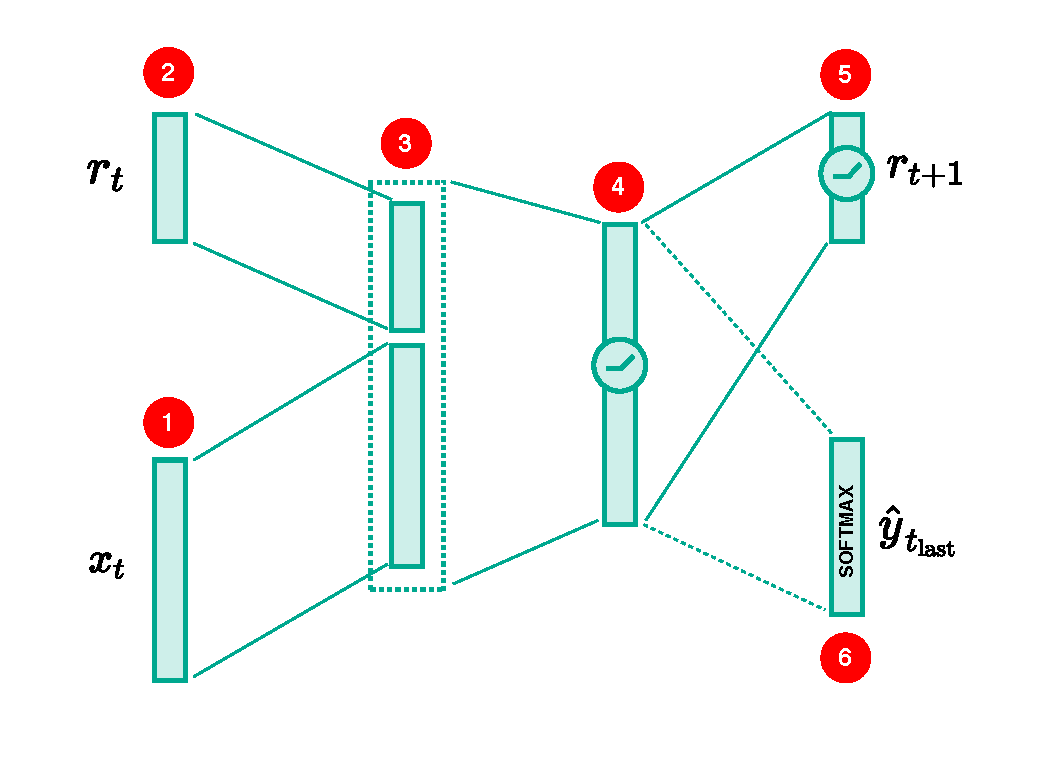
\includegraphics[width=0.48\textwidth]{sketch/s2_network}
     }
     \hfill
     \subfloat[Deep cell\label{fig:s3_network}]{%
       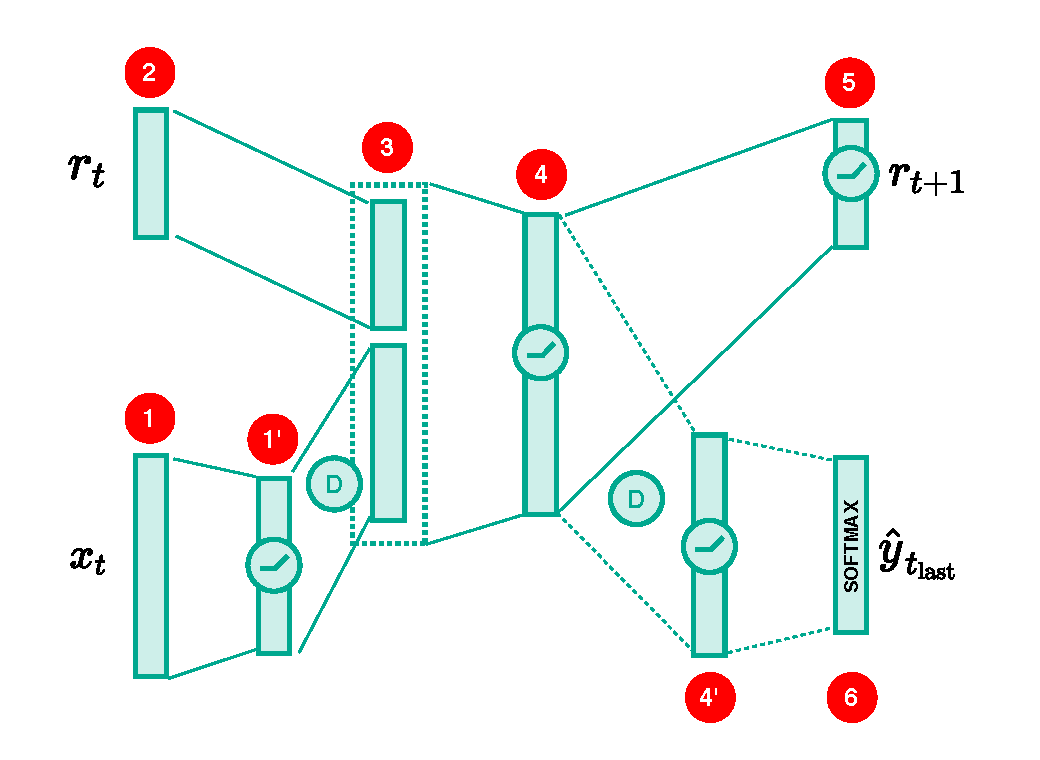
\includegraphics[width=0.48\textwidth]{sketch/s3_network}
     }
\caption{Shallow and Deep Cell Architecture}
\end{figure}

As shown in \addfigure{\ref{fig:s2_network}}, \rnncell{Shallow} cell first concatenates  input $\patvector{x}_t$  \circled{1} and recurrent input $\patvector{r}_t$  \circled{2} at layer \circled{3} as one vector before computing $\patvector{a}_t^{(4)} $ of layer \circled{4}. Then,  the next recurrent input $\patvector{r}_{t+1}$ \circled{5}	 is derived from $\patvector{a}_t^{(4)}$. In the last step $t_{\text{last}}$, the raw output $\patvector{h}$ is computed from $\patvector{a}^{(4)}_{t_{\text{last}}}$ and applied to softmax function to compute class probabilities $\patvector{\hat{y}}$ \circled{6}.



\subsection{Deep Cell Architecture}
%\begin{figure}[!htb]
%\centering
%
%\end{figure}

\addfigure{\ref{fig:s3_network}} illustrates the architecture of  \rnncell{Deep} cell. It can be viewed as  an extension of the Shallow cell with  2 additional layers, namely \circled{1'} and \circled{4'}.  The ideas of introducing the layers are to let \circled{1'} learn representations of the problem, while \circled{4} can focus on combining information from past and current step, which enables \circled{4'} to compute more fine-grained decision probabilities. Dropout is applied at $\patvector{a}^{(1')}_{\cdot}$, and $\patvector{a}^{(4)}_{t_\text{last}}$ for computing $\patvector{a}^{(4')}$.

\begin{figure}[!htb]
\centering

\subfloat[DeepV2\label{fig:deep_4l_network}]{%
       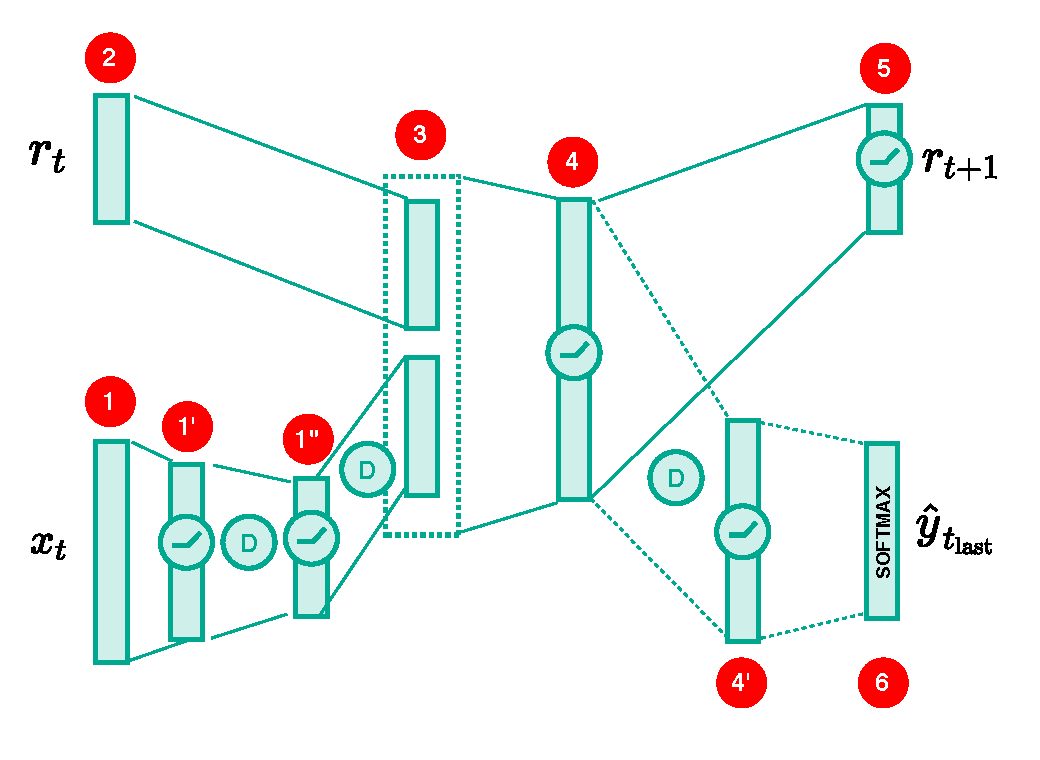
\includegraphics[width=0.48\textwidth]{sketch/deep_4l_network}
     }
     \hfill
     \subfloat[ConvDeep\label{fig:convdeep_4l_network}]{%
       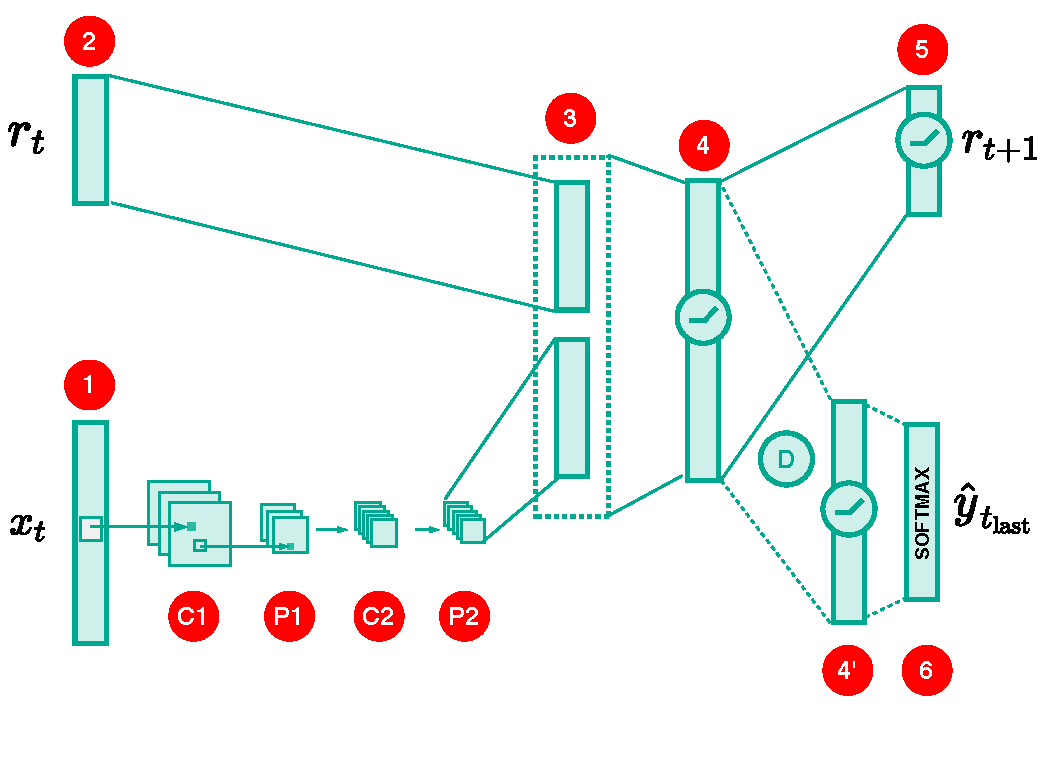
\includegraphics[width=0.48\textwidth]{sketch/convdeep_4l_network}
     }

\caption{DeepV2 and ConvDeep Cell Architecture}
\label{fig:deep_conv_arch}
\end{figure}
%
%
%
%\begin{figure}[!htb]
%\centering
%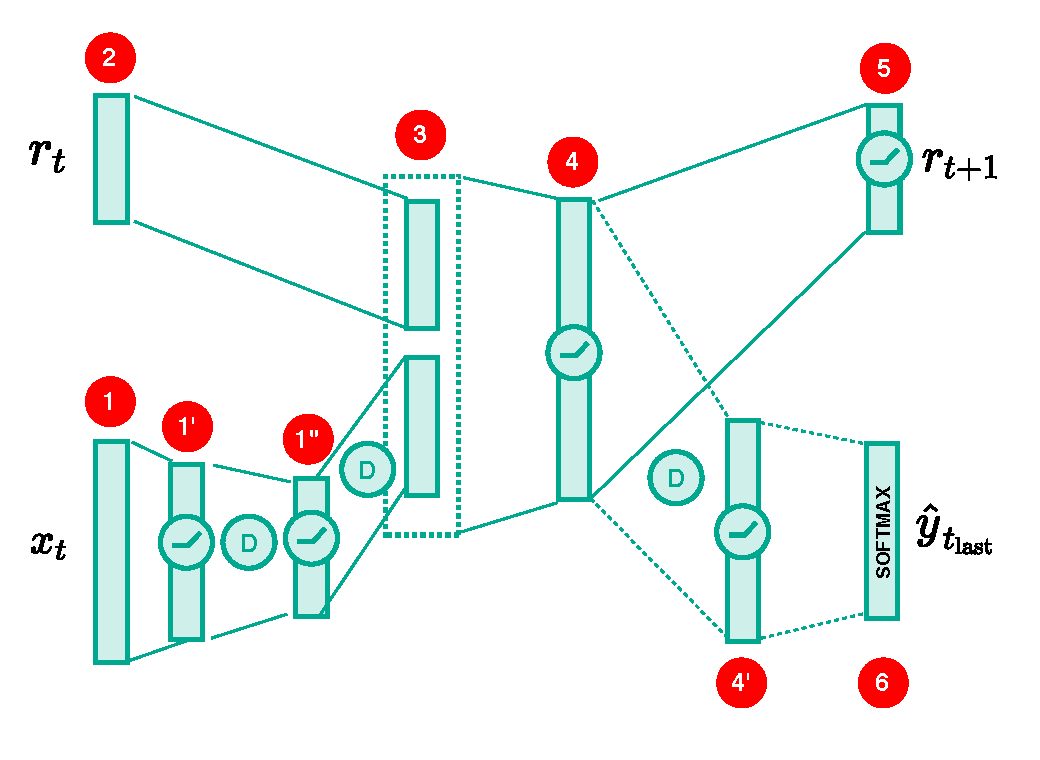
\includegraphics[width=0.6\textwidth]{sketch/deep_4l_network}
%\caption{DeepV2 Cell Architecture}
%\label{fig:deep_4l_network}
%\end{figure}
%
%
%\begin{figure}[!htb]
%\centering
%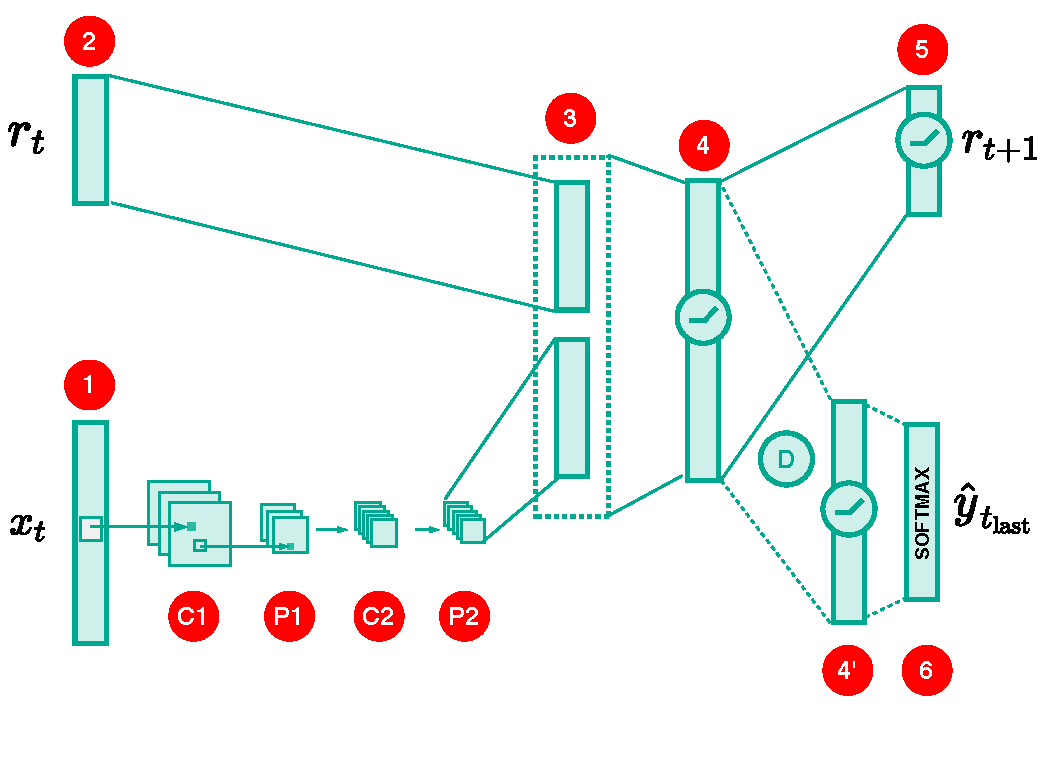
\includegraphics[width=0.6\textwidth]{sketch/convdeep_4l_network}
%\caption{ConvDeep Architecture}
%\label{fig:convdeep_4l_network}
%\end{figure}

Two variations of \rnncell{Deep} cell are also experimented, namely \rnncell{DeepV2} and \rnncell{ConvDeep}, shown on \addfigure{\ref{fig:deep_conv_arch}}. The former has one additional layer \circled{1"} with dropout regularization  between \circled{1'}. On the other hand, the latter replaces fully connected layers between \circled{1} and \circled{3} with 2 convolutional and max pooling layers, \Big[\circled{C1}, \circled{P1}\Big] and \Big[\circled{C2},\circled{P2}\Big].




\section{Setup}\label{sec:setup}
 
 I implemented experiments using TensorFlow\footnote{\url{http://tensorflow.org/}}.  weights $w_{ij} \in \patmatrix{W}$ and biases $b_{j} \in \patvector{b}$ are initialized as follows:
\begin{align*}
	w_{ij} &\sim \Psi( \mu=0, \sigma =0.1, [-2\sigma, 2\sigma]) \\
	b_{j} &= \ln(e^{0.01} - 1)
\end{align*}
where $\Psi(\cdot)$ denotes Truncated Normal Distribution with valid region between $[-2\sigma, 2\sigma]$.

%TODO : Figure normal distribution vs trucated

Activations $\patvector{a}^{(l)}_\cdot$ of layer $l$ is calculated using :
\begin{align*}
	\patvector{h}^{(l)}  &=  	\patmatrix{W}^T \patvector{a}^{(l-1)} - \sigma_{s}(\patvector{b}) \\
	\patvector{a}^{(l)}  &=  	\sigma_{r} (	\patvector{h}^{(l)} )
\end{align*}

where
\begin{align*}
	\sigma_{r} (h_j) &= \max(0, h_j)  \tag{ReLU function}\\
	\sigma_{s} (b_j) &= \log(1+\exp b_j) \tag{Softplus function}
\end{align*}
%TODO : Figure softplus vs relu

The reason of using $\sigma_{s} (b_j)$ for bias term is due to the non positive bias assumption of DTD. Moreover, $\sigma'_{s} (b_j)$ is $(0, \infty)$, as a result the network has more flexibility to adjust decision through back-propagation rather than using $\sigma_{r} (b_j)$. With this setting, the initial value of bias term  $\sigma_{s}(b_j)$ is then 0.01.

Speaking about training methodology, I use Adam\cite{KingmaAdamMethodStochastic2014} optimizer to train networks. Preliminary study shows that relevance heatmaps from networks trained by Adam are less noisy than the ones from other optimizers, such as  Stochastic Gradient Descent(SGD). Number of epochs is set to 200, while dropout probability is 0.5 and batch size is 50.  
Learning rate is not fixed as it is likely that different network architectures requires different value to achieve good performance, hence left adjustable. Table \ref{tab:hyper_summary} summaries the setting of hyperparameters.

%TODO: Heatmaps SGD, RMSProp, Adam
 
 \begin{table}[!htb]
\centering
\begin{tabular}{l|r}
\textbf{Hyperparameter} & \multicolumn{1}{l}{\textbf{Value}} \\ \hline
Optimizer               & Adam                               \\
Epoch     & 200                                \\
Dropout Probability     & 0.5                                \\
Batch size              & 50                                
\end{tabular}
\caption{Hyperparameter Summary}
\label{tab:hyper_summary}
\end{table}
 
Traditionally, number of neurons in each layer ($n^{(l)}$) is  another hyperparameter that we can adjust. However, as the goal is to compare relevance heatmaps from different architectures, those numbers are fixed and chosen in such a way that total number of variables in each architecture are equivalent. \addfigure{\ref{fig:neuron_numbers}} illustrates the details of the settings.

\begin{figure}[!htb]
\centering
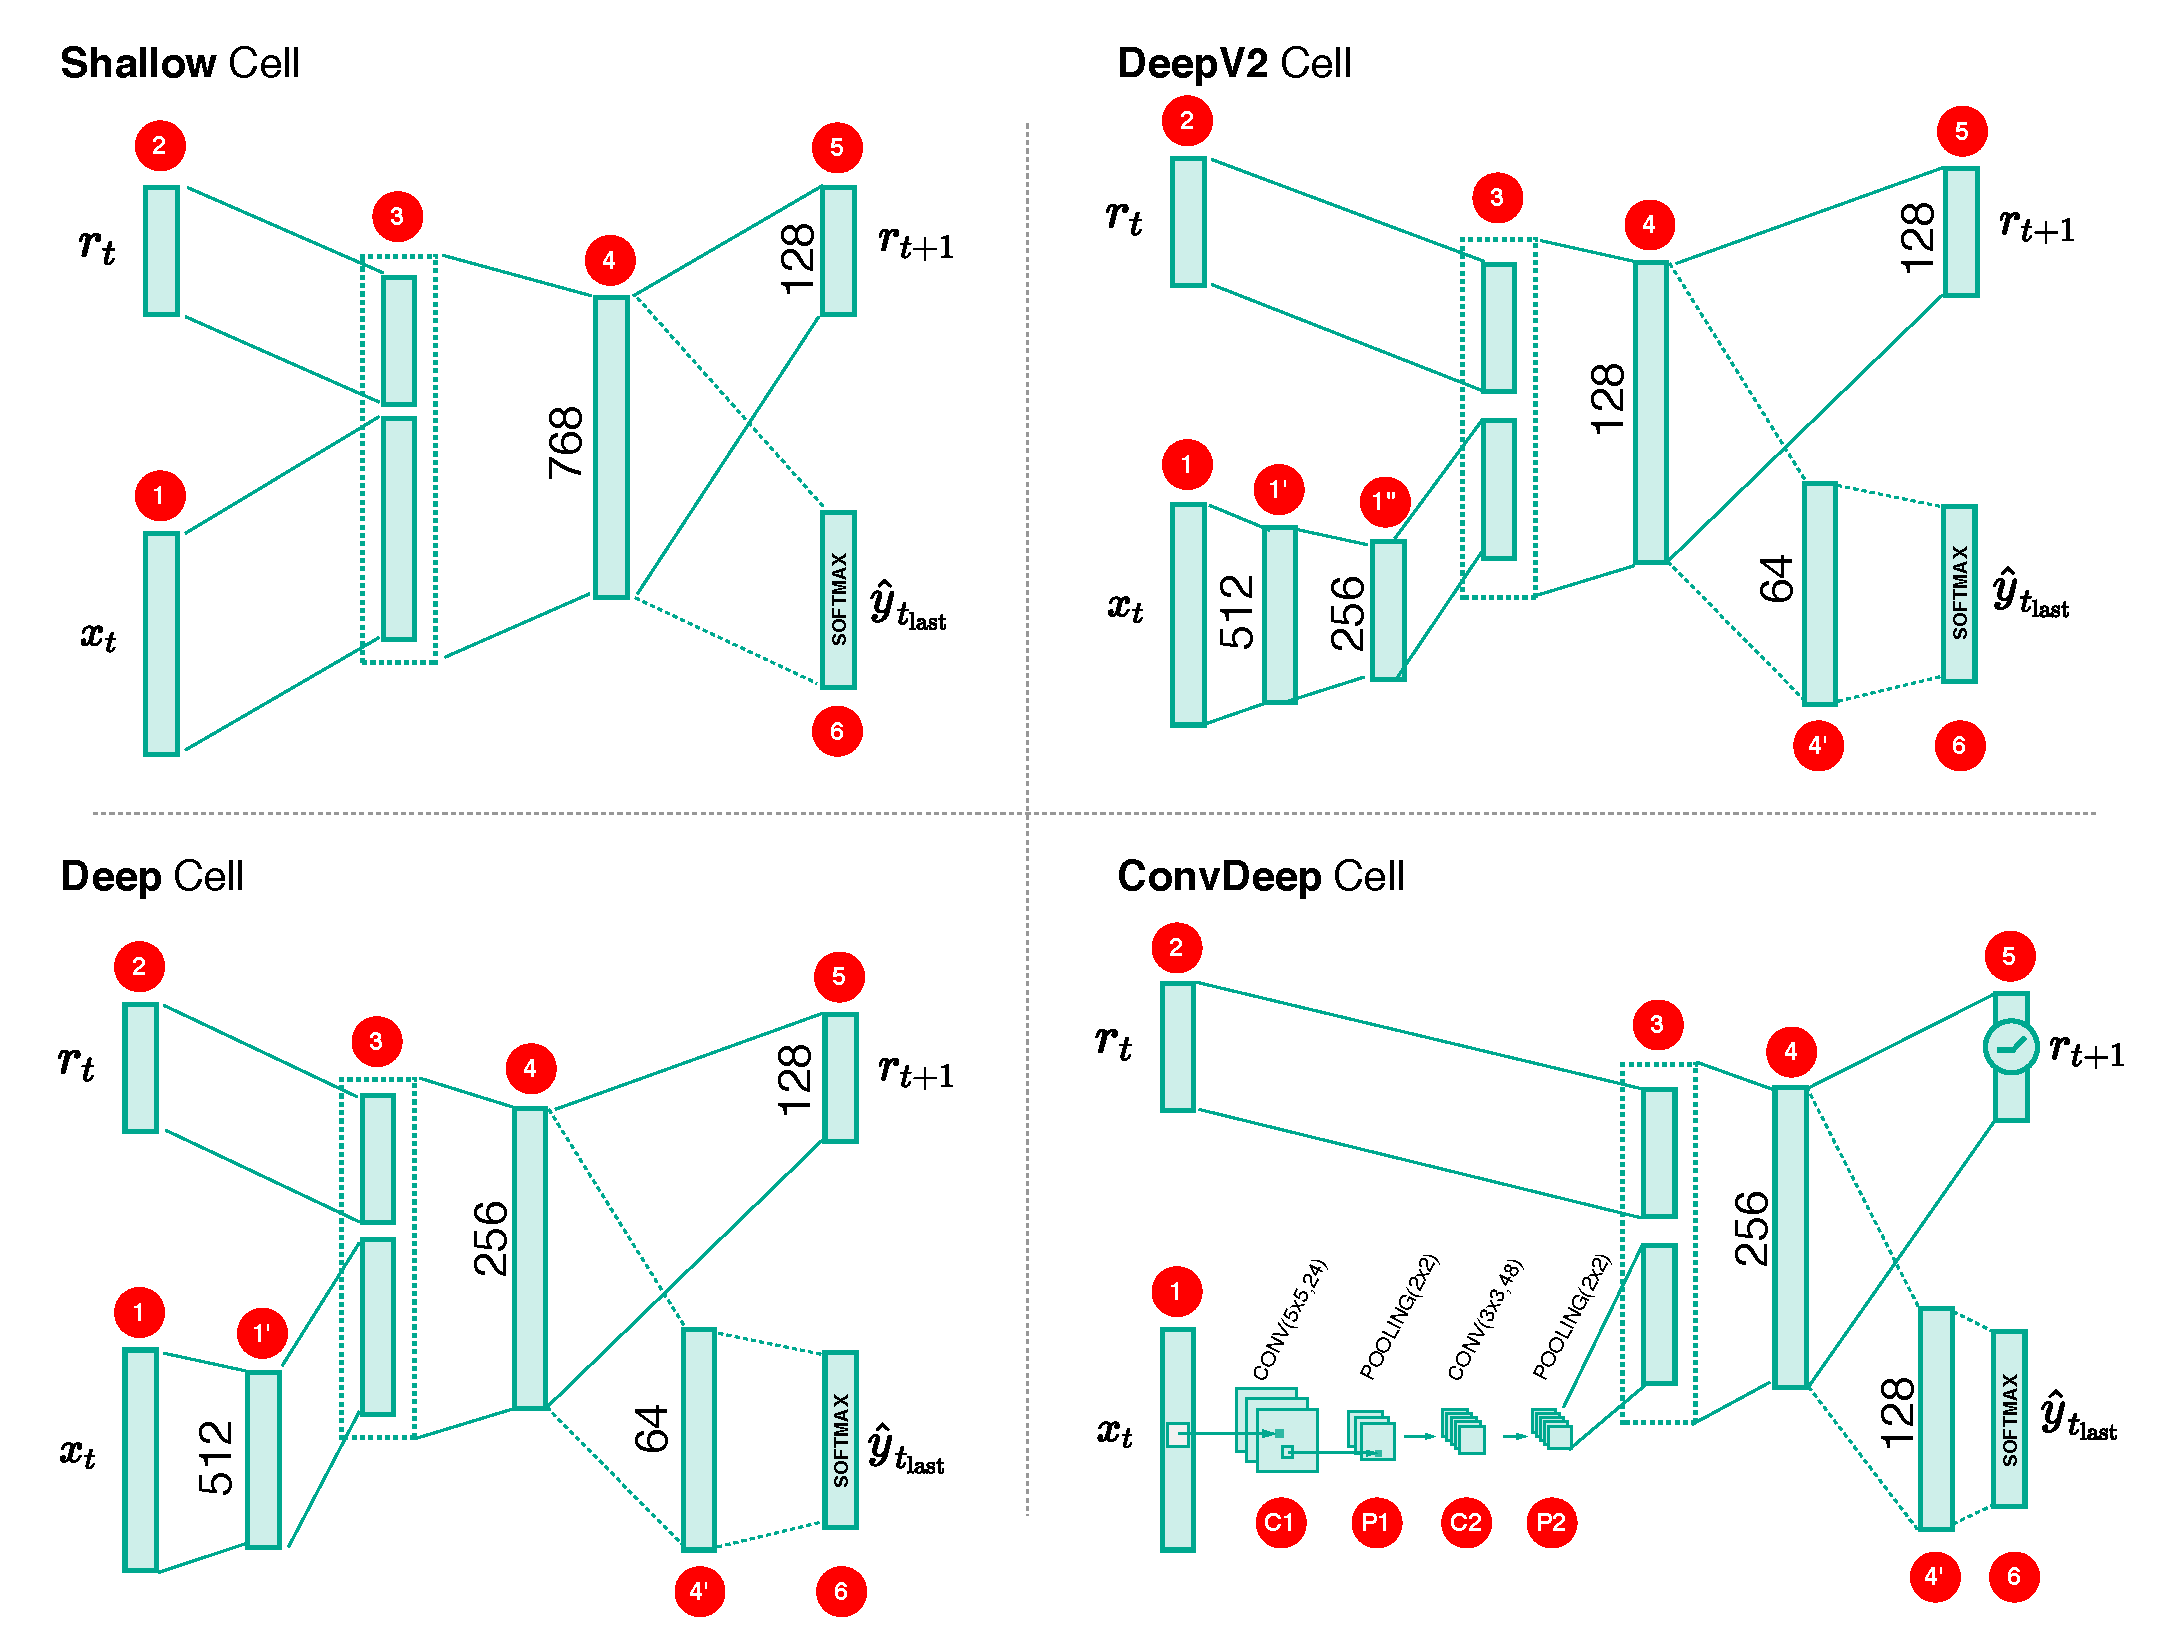
\includegraphics[width=\textwidth]{sketch/neuron_numbers}
\caption{Number of neurons in each layer for each cell architecture}
\label{fig:neuron_numbers}
\end{figure}


\begin{itemize}
	\item \textbf{Shallow Cell} 
$$\{ n^{(4)}\} = \{ 768 \}$$
	\item \textbf{Deep Cell} 
$$\{ n^{(1')}, n^{(4)}, n^{(4')} \} = \{ 512, 256, 64 \}$$
	\item \textbf{DeepV2 Cell} 
$$\{ n^{(1')}, n^{(1")}, n^{(4)}, n^{(4')} \} = \{ 512, 256, 128, 64 \}$$
	\item \textbf{ConvDeep Cell} : 
\begin{align*}
	\{ n^{(C1)}, n^{(P1)} \} &= \{ CONV(5\text{x}5, 24), POOL(2\text{x}2) \} \\
		\{ n^{(C2)}, n^{(P2)} \} &= \{ CONV(3\text{x}3, 48), POOL(2\text{x}2) \} \\
			\{  n^{(4)}, n^{(4')} \} &= \{ 256, 128 \}
\end{align*}
where $CONV(x,y)$ is a convolutional operator with $y$ filters whose kernel size is $\mathbb{R}^{x}$. Similarly, $POOL(x)$ is a pooling operator  with kernel size $\mathbb{R}^{x}$.


\end{itemize}

Noting that, $n^{(5)}$ is set at 128 for all architectures and 0 when the sequence length of the problem is 1. $n^{(6)}$ is equal to the number of categories of a problem, for example $n^{(6)} = 10 $ MNIST. Table \ref{tab:variable_architecture} shows the total numbers of variables in details.

\renewcommand{\arraystretch}{1.2}
\begin{table}[h]
\centering
\begin{tabular}{l|c|c|c|c|}
\cline{2-5}
                                                 & \multicolumn{4}{c|}{\textbf{Sequence Length}} \\ \hline
\multicolumn{1}{|l|}{\textbf{Cell Architecture}} & 1         & 4         & 7         & 14        \\ \hline
\multicolumn{1}{|l|}{\rnncell{Shallow}}                    & 610570    & 355722    & 291210    & 248202    \\ \hline
\multicolumn{1}{|l|}{\rnncell{Deep}}                       & 550346    & 314954    & 271946    & 243274    \\ \hline
\multicolumn{1}{|l|}{\rnncell{DeepV2}}                    & 575050    & 306890    & 263882    & 235210    \\ \hline
\multicolumn{1}{|l|}{\rnncell{ConvDeep}}                   & 647594    & 283178    & 197162    & 197162    \\ \hline
\end{tabular}
\caption{Total variables in each architecture and sequence length}
\label{tab:variable_architecture}
\end{table}


Lastly, as the quality of relevance heatmap depending on performance of the model, the minimum classification accuracy is set as in Table  \ref{tab:min_acc}. 

\begin{table}[h]
\centering
\begin{tabular}{ll}
\multicolumn{1}{l|}{\textbf{Dataset}} & \textbf{Minimum Accuracy} \\ \hline
\multicolumn{1}{l|}{MNIST}            & \multicolumn{1}{r}{0.98}  \\
\multicolumn{1}{l|}{Fashion-MNIST}    & \multicolumn{1}{r}{0.85}  \\
%\multicolumn{1}{l|}{UFI Cropped}                                       &                         \dots
\end{tabular}
\caption{Classification Accuracy Criteria}
\label{tab:min_acc}
\end{table}

% TODO : Hyper hopt Hyperopt

\section{Experiment 1 : Sequence Classification}

\subsection{Problem Formulation}
To demonstrate how well RNNs can distribute relevant quantities to input space, I formulated an artificial classification problem in which each image sample $\x$ is column-wise split into non-overlapping $(\x_t)_{t=1}^{T}$.  The RNN classifier needs to summarize information from the sequence $(\x_t)_{t=1}^{T}$ to answer what is the class of $\x$.   

\addfigure{\ref{fig:artificial_problem}} illustrates the setting. Here, a MNIST sample $ \patvector{x} \in \mathbb{R}^{28,28}$ is divided to a sequence of $( \patvector{x}_t \in   \mathbb{R}^{28,7} )_{t=1} ^ 4$. At time step $t$, $\patvector{x}_t$ is presented to the RNN classifier which yields recurrent input $\patvector{r}_{t+1}$ for the next step. For the last step $T$, in this example $T = 4$, the RNN classifier computes $f(\x) \in \mathbb{R}^{10}$ and the class that $\x$ belongs to. 

 \begin{figure}[!hbt]
\centering
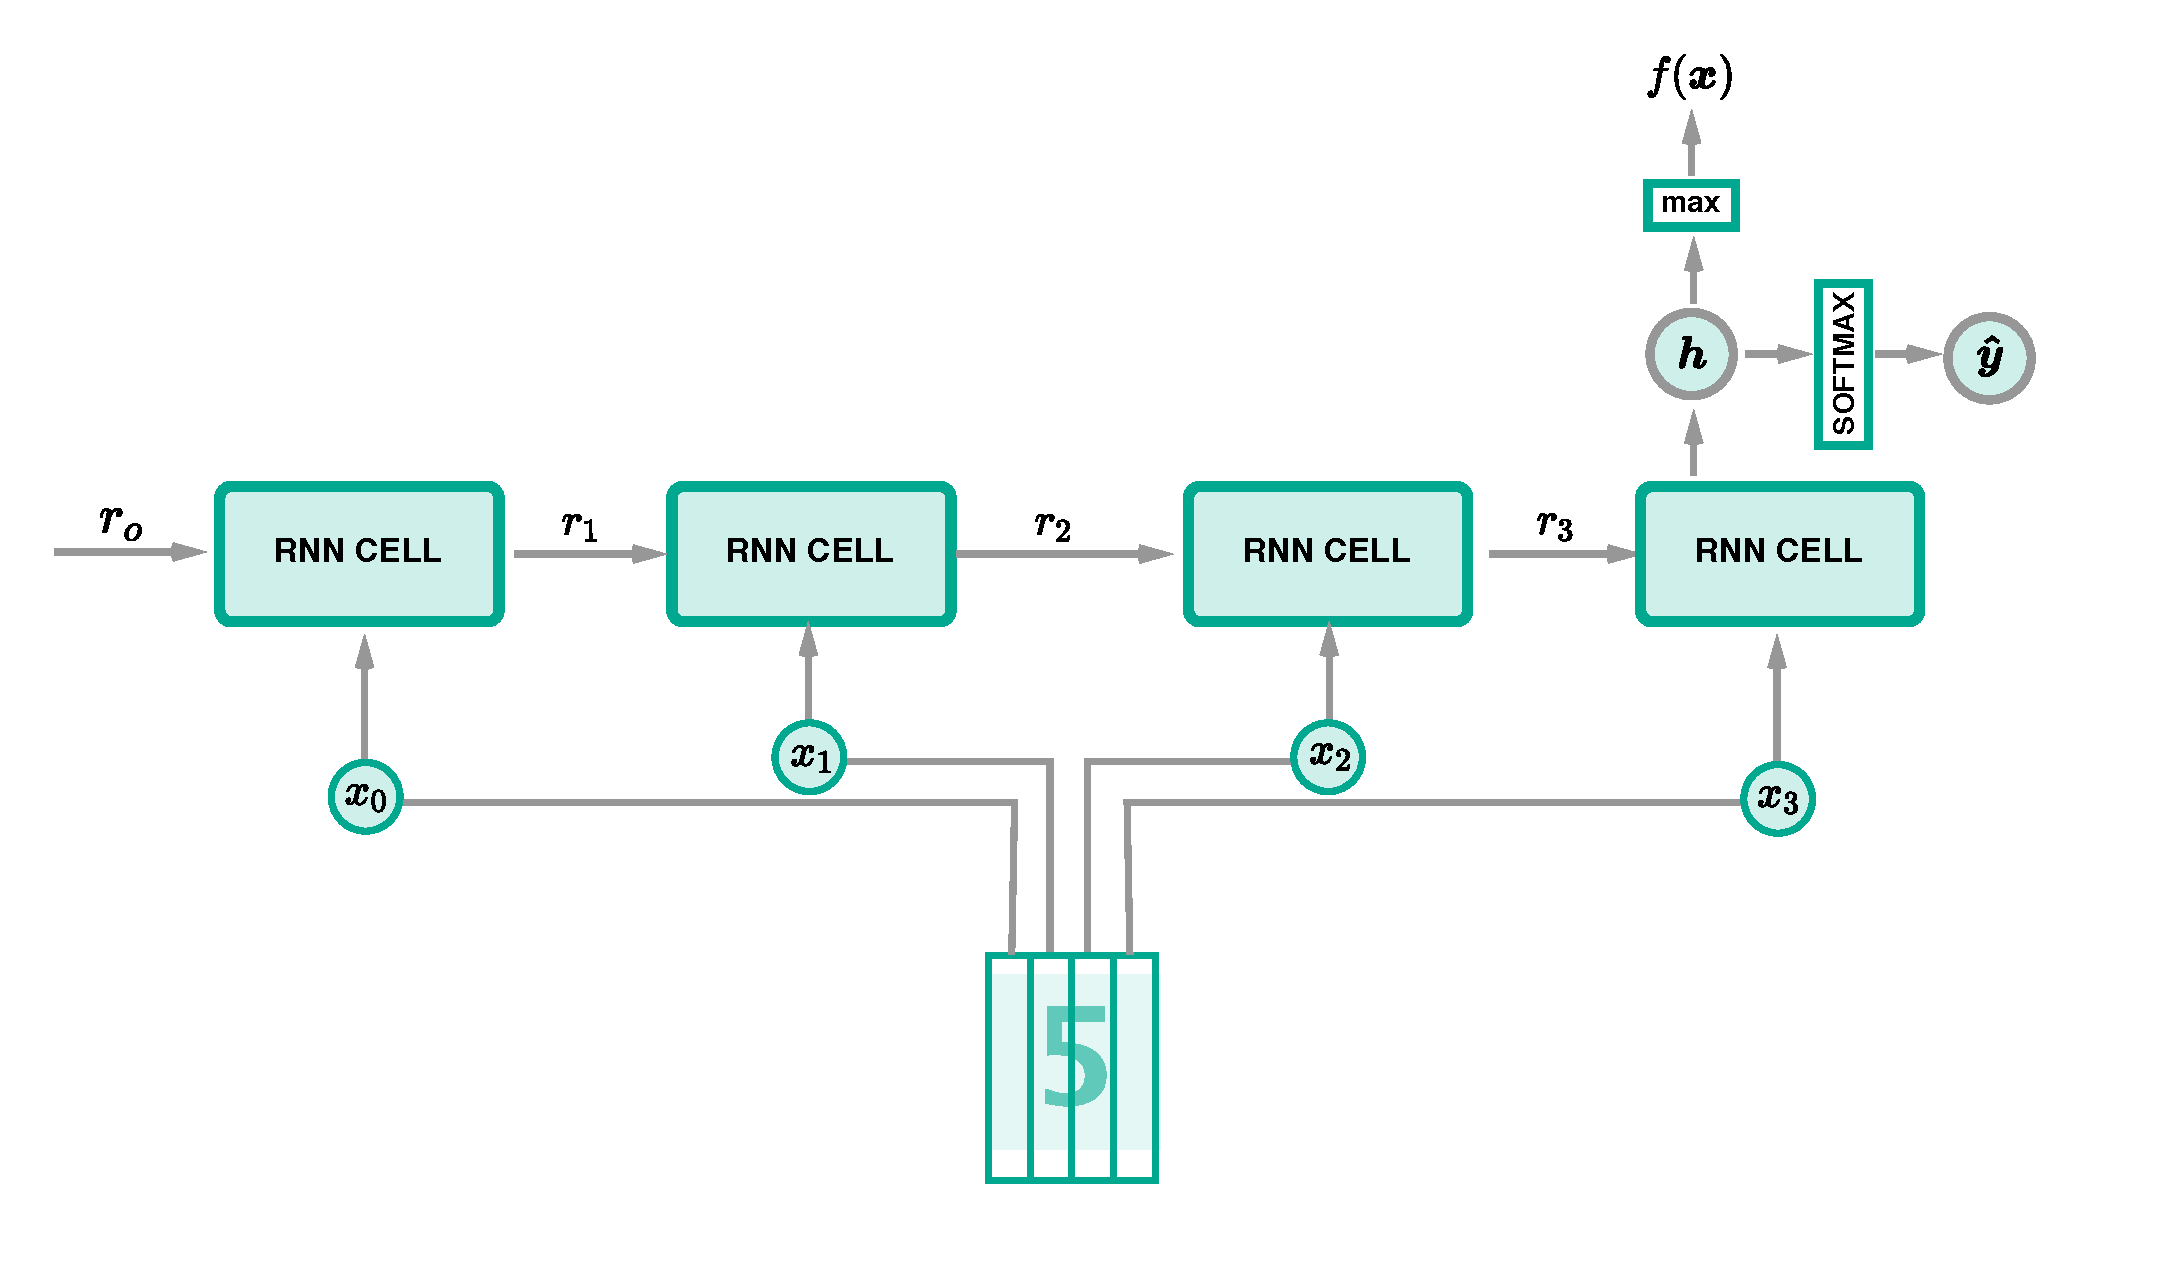
\includegraphics[width=0.9\textwidth]{sketch/artificial_problem}
\caption{General setting of RNN classifiers in this thesis} 
\label{fig:artificial_problem}
\end{figure}

 Denote $g_r$ and $g_{f}$ function that the RNN  with parameters $\boldsymbol{\theta}$ uses to compute $\patvector{r}_{t+1}$ and $f(\x)$ respectively. The overall computation can be summarized as follows: 
 \begin{align*}
 	\patvector{r}_{t+1} &= g_r(\patvector{\theta}, \patvector{x_t}, \patvector{r_t}) \\
 	 &\ \ \vdots\\
f(\x) &= g_{h}(\patvector{\theta}, \patvector{x}_{t_{\text{last}}},  \patvector{r}_{t_{\text{last}}}) \\
 	\patvector{\hat{y}} &= \text{softmax}(f(\x)),
 \end{align*}
 where $\patvector{\hat{y}}$ is the class probabilities and $\patvector{r}_0 = \patvector{0}$.   To explain the model,  $R(\x)$ is set to the value of $f(\x)$ that is corresponding to the true target class.
 
 \todo{figure show how R(x) is set?}
 
 
\renewcommand{\arraystretch}{1.5}
\begin{table}[h]
\centering
\begin{tabular}{l|l|l|l|l|}
\cline{2-4}
                                            & \multicolumn{3}{c|}{Sequence Length}                                                               \\ \hline
\multicolumn{1}{|c|}{Dataset}               & \multicolumn{1}{c|}{1} & \multicolumn{1}{c|}{4} & \multicolumn{1}{c|}{7}  \\ \hline
\multicolumn{1}{|l|}{MNIST / FashionMNIST} &        $ \mathbb{R}^{28,28}  $              &          $ \mathbb{R}^{28,7}  $               &         $ \mathbb{R}^{28,4}  $                            \\ \hline
%\multicolumn{1}{|l|}{UFI-Cropped}           &                        &                        &                        &                         \\ \hline
%\multicolumn{1}{|l|}{}                      &                        &                        &                        &                         \\ \hline
\end{tabular}
\caption{Dimensions of $\patvector{x}_t$ for each dataset and sequence length}
\label{tab:seq-length}

\end{table}
\renewcommand{\arraystretch}{1}

%In this section, I am going to present what I have  found from experiments. First, I am going to discuss results from MNIST and then move on to ones from Fashion-MNIST. Moreover, I will use \rnncellseq{CELL\_NAME}{SEQ} convention to denote a RNN network with CELL\_NAME cell trained on a sequence length SEQ. For example, \rnncellseq{Deep}{7} means a RNN with Deep cell architecture trained on data whose $\patvector{x}^{(\alpha)}$ is a sequence of length 7.
%TODO : More introduction

\subsection{Result}
I began this preliminary experiment  with Shallow and Deep architecture. They were trained on MNIST and FashionMNIST with sequence length $ SEQ = \{1, 4, 7\}$. Table \ref{tab:seq-length} shows dimensions of $\patvector{x}_t$ for different sequence length and Table \ref{tab:mnist_model_acc} summaries accuracy of the trained models. To simplify the manuscript, I am going to use \textit{\rnncellseq{ARCHITECTURE}{SEQ}} convention to denote a RNN with \textit{ARCHITECTURE} trained on sequence length \textit{SEQ}. For example, \rnncellseq{Deep}{7} means a  Deep RNN architecture trained on $(\x_t \in \mathbb{R}^{28,4} )_{t=1}^{7}$.


\begin{table}[]
\centering
\begin{tabular}{lrr}
\textbf{}                  & \multicolumn{1}{c}{\textbf{Shallow}} & \multicolumn{1}{c}{\textbf{Deep}} \\ \hline
\multicolumn{1}{l|}{SEQ-1} & xx.xx\%                              & xx.xx\%                           \\
\multicolumn{1}{l|}{SEQ-4} & xx.xx\%                              & xx.xx\%                            \\
\multicolumn{1}{l|}{SEQ-7} & xx.xx\%                              & xx.xx\%
\end{tabular}
\caption{Model Accuracy}
\label{tab:mnist_model_acc}
\end{table}


 \begin{figure}[h]
\centering
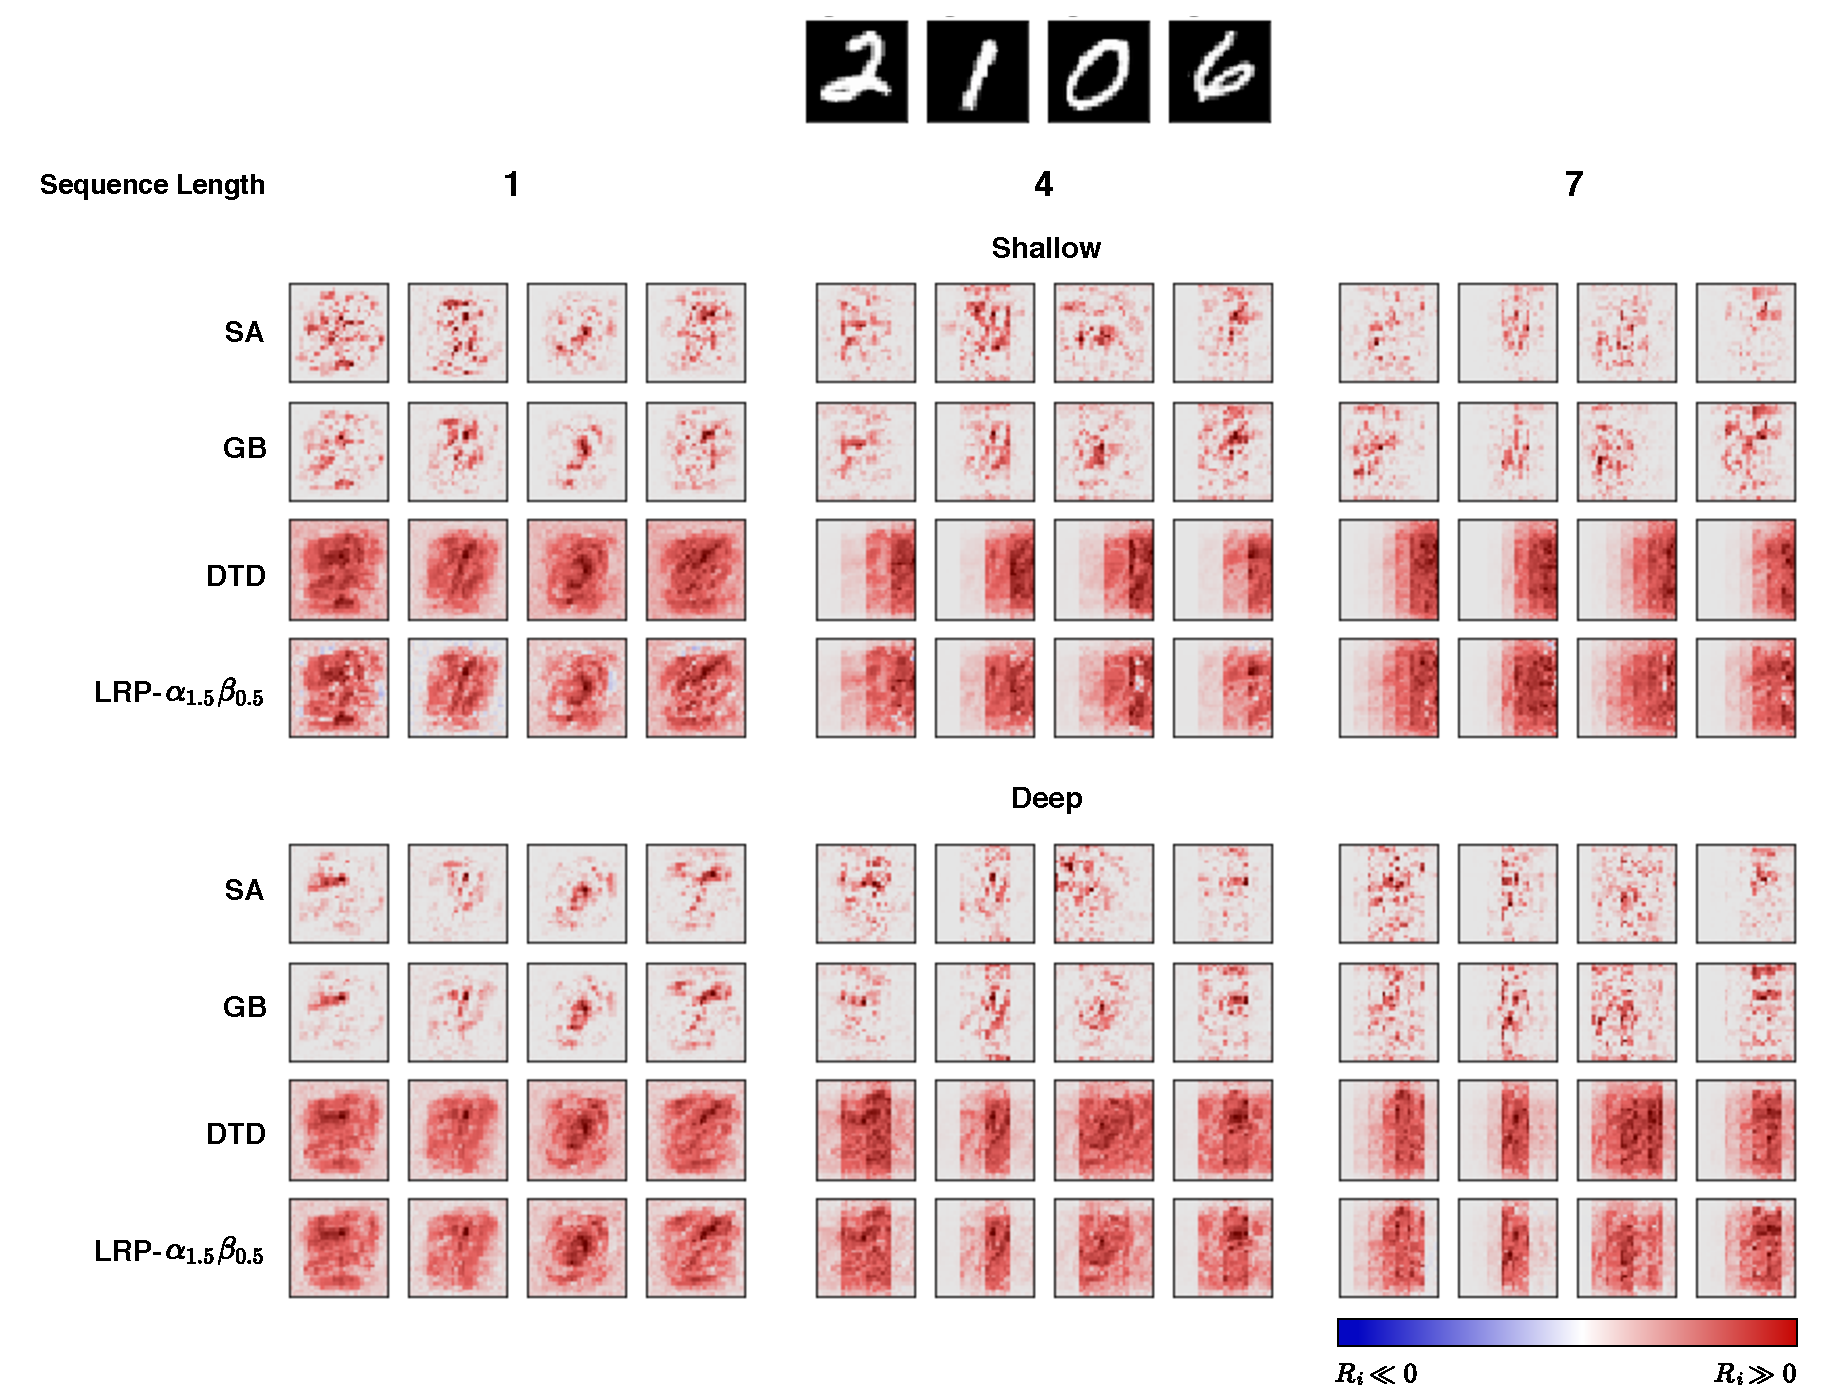
\includegraphics[width=0.8\textwidth]{sketch/mnist_experiment}
\caption{Relevance heatmaps from Shallow and Deep Cell trained on MNIST with different sequence lengths}
\label{fig:mnist_experiment}
\end{figure}


\addfigure{\ref{fig:mnist_experiment}} shows relevance heatmaps from Shallow and Deep architecture trained on MNIST.  We can see general characteristics of each explanation technique. In particular, sensitivity analysis(SA) and guided backprop(GB) heatmaps are sparse, while the ones from deep Taylor decomposition(DTD) are more diffuse throughout $\x$.  When applying these techniques to \rnncellseq{Shallow}{1}  and \rnncellseq{Deep}{1}, the relevance heatmaps look similar regardless of the architectures.  As the sequence length is increased, SA and GB heatmaps are still almost identical  for \rnncellseq{Shallow}{4,7} and \rnncellseq{Deep}{4,7}. However, this is not the case for DTD.  From the figure, we can see that \rnncellseq{Shallow}{4,7} and  \rnncellseq{Deep}{4,7} return significantly different relevance heatmaps from DTD method.  In particular,  \rnncellseq{Shallow}{4,7} 's heatmaps are mainly concentrated on the right part of $\x$ associating to last time steps, while  \rnncellseq{Deep}{4,7}'s ones are appropriately highlighted at the actual content area of $\x$.


 \begin{figure}[h]
\centering
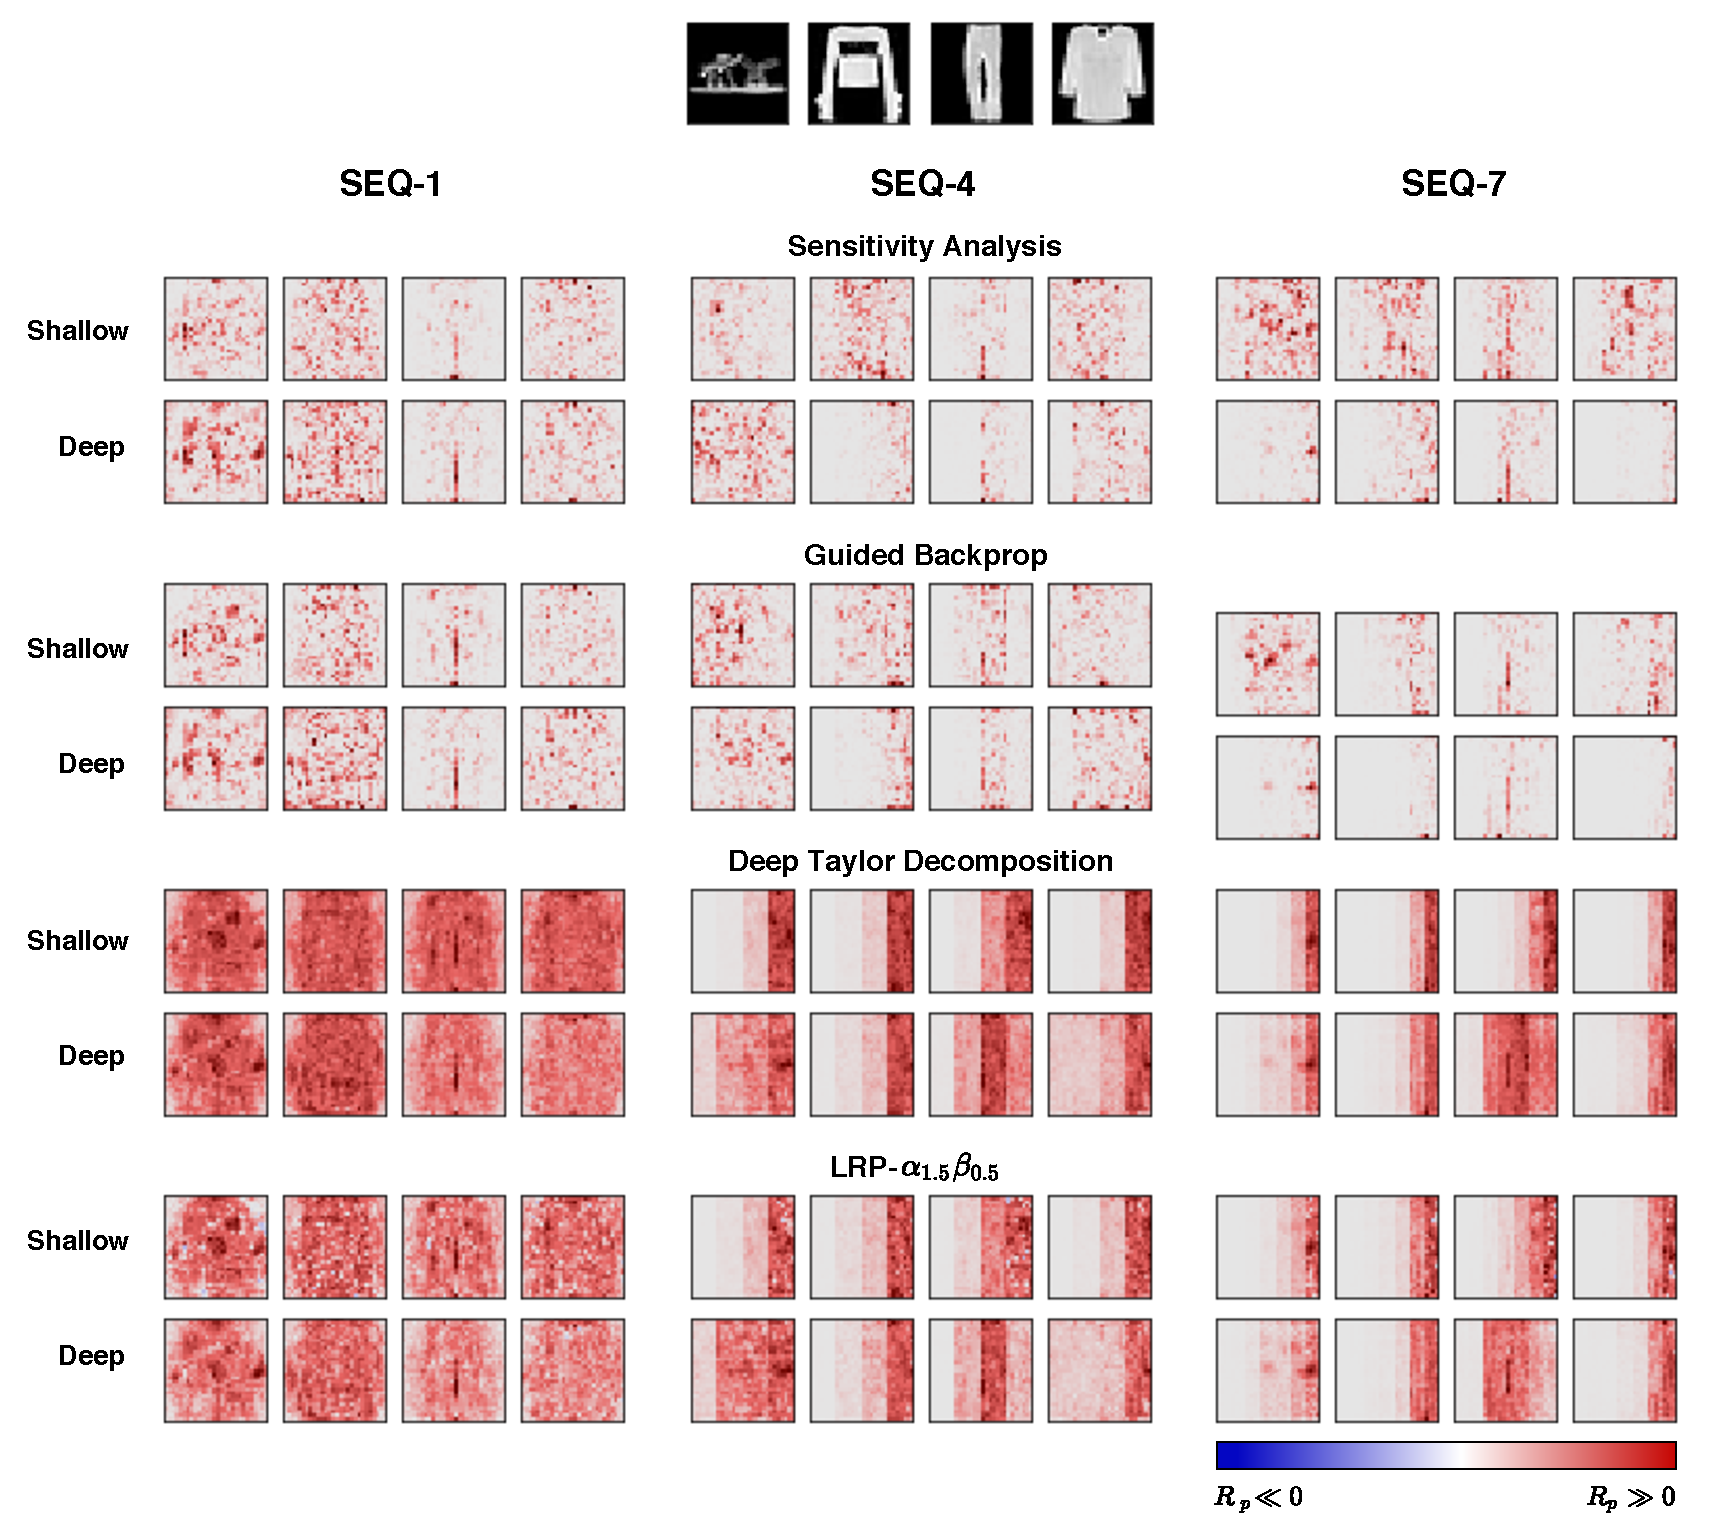
\includegraphics[width=0.8\textwidth]{sketch/fashion_mnist_experiment}
\caption{Relevance heatmaps from Shallow and Deep Cell trained on FashionMNIST with different sequence lengths}
\label{fig:fashion_mnist_experiment}
\end{figure}

Relevance heatmaps of Shallow and Deep architecture trained on  FashionMNIST  are shown on \addfigure{\ref{fig:fashion_mnist_experiment}}. Similar to MNIST, we do not see any remarkable difference on SA and GB heatmaps of the two architectures : only that \rnncellseq{Deep}{4,7} produces slightly more sparse heatmaps. The wrong concentration issue of DTD  seems to appear on both \rnncellseq{Shallow}{4,7}'s and \rnncellseq{Deep}{4,7}'s heatmaps although we can still see correct highlight from Deep architecture on some samples. For example, the trouser sample, we can see  that \rnncellseq{Deep}{4,7} architecture manage to distribute high relevance scores to area of the trouser.






 \begin{figure}[ht!]
\centering
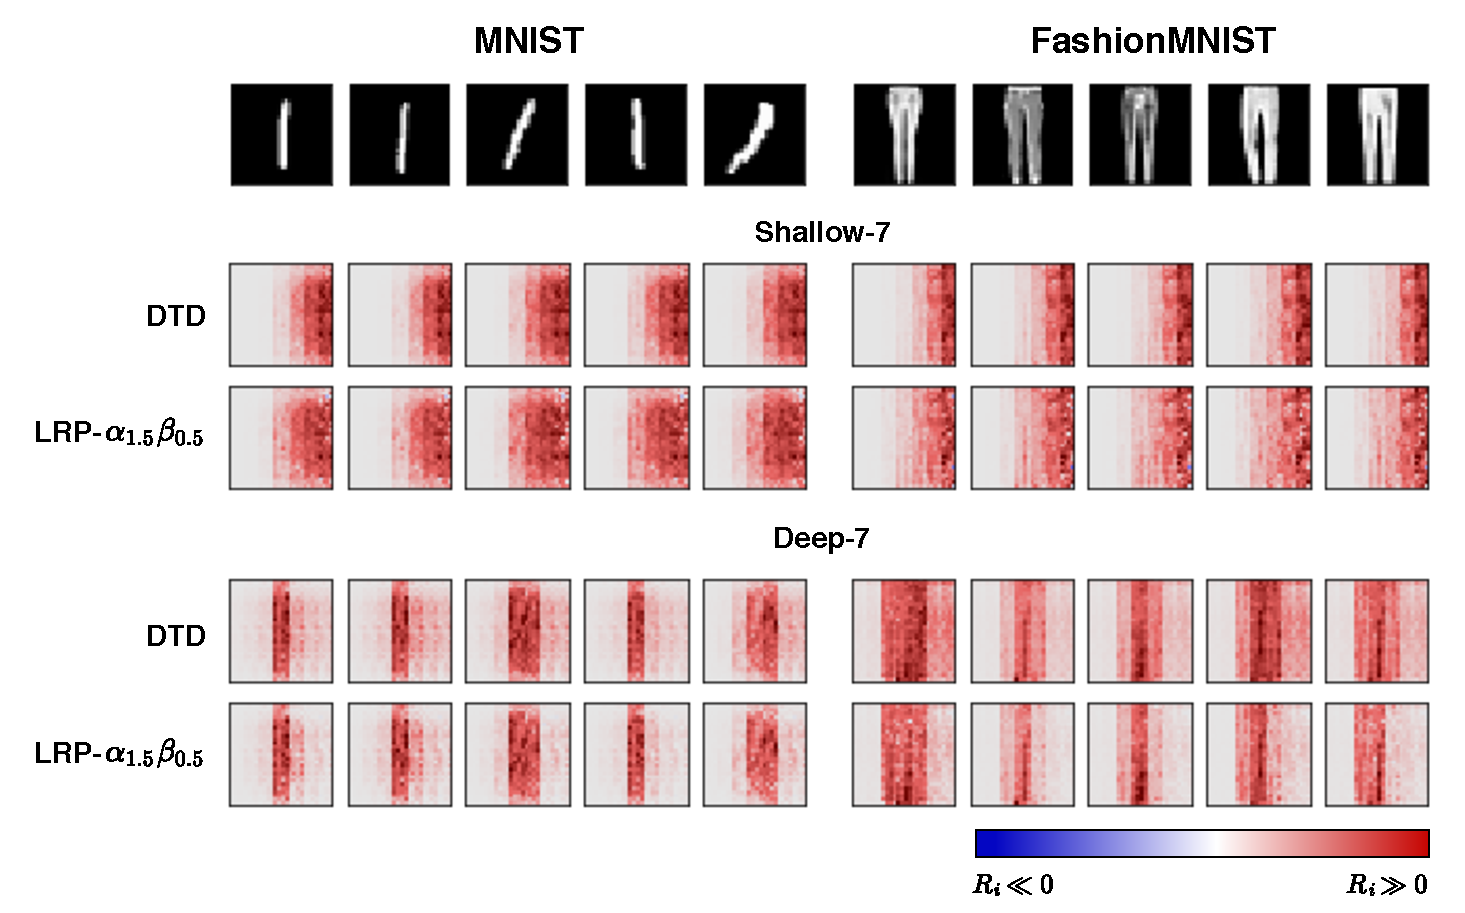
\includegraphics[width=\textwidth]{sketch/class_1_comparison}
\caption{DTD relevance heatmaps of MNIST \textit{Class 1} and FashionMNIST \textit{Class Trouser} samples from \rnncellseq{Shallow}{7} and \rnncellseq{Deep}{7} }\\
\label{fig:class_1_comparison}
\end{figure}

\addfigure{\ref{fig:class_1_comparison}} presents relevance heatmaps of MNIST \textit{Class 1} and FashionMNIST \textit{Class Trouser} samples. These samples were chosen to emphasize the impact of RNN architecture on DTD explanation. In particular,  these samples have $\x_{t'}$ containing features  primarily locating at the center, or middle of the sequence, hence appropriate relevance heatmaps should be highlighted at $\x_{t'}$ and possibly its neighbors.  As expected, we can see \rnncellseq{Deep}{7} produces sound results in which the  heatmaps have high intensity value where $\x_{t'}$ approximately locate, while \rnncellseq{Shallow}{7} mainly assigns relevance quantities to $\x_{t}$ for $t \approx T$.


 \begin{figure}[h]
\centering
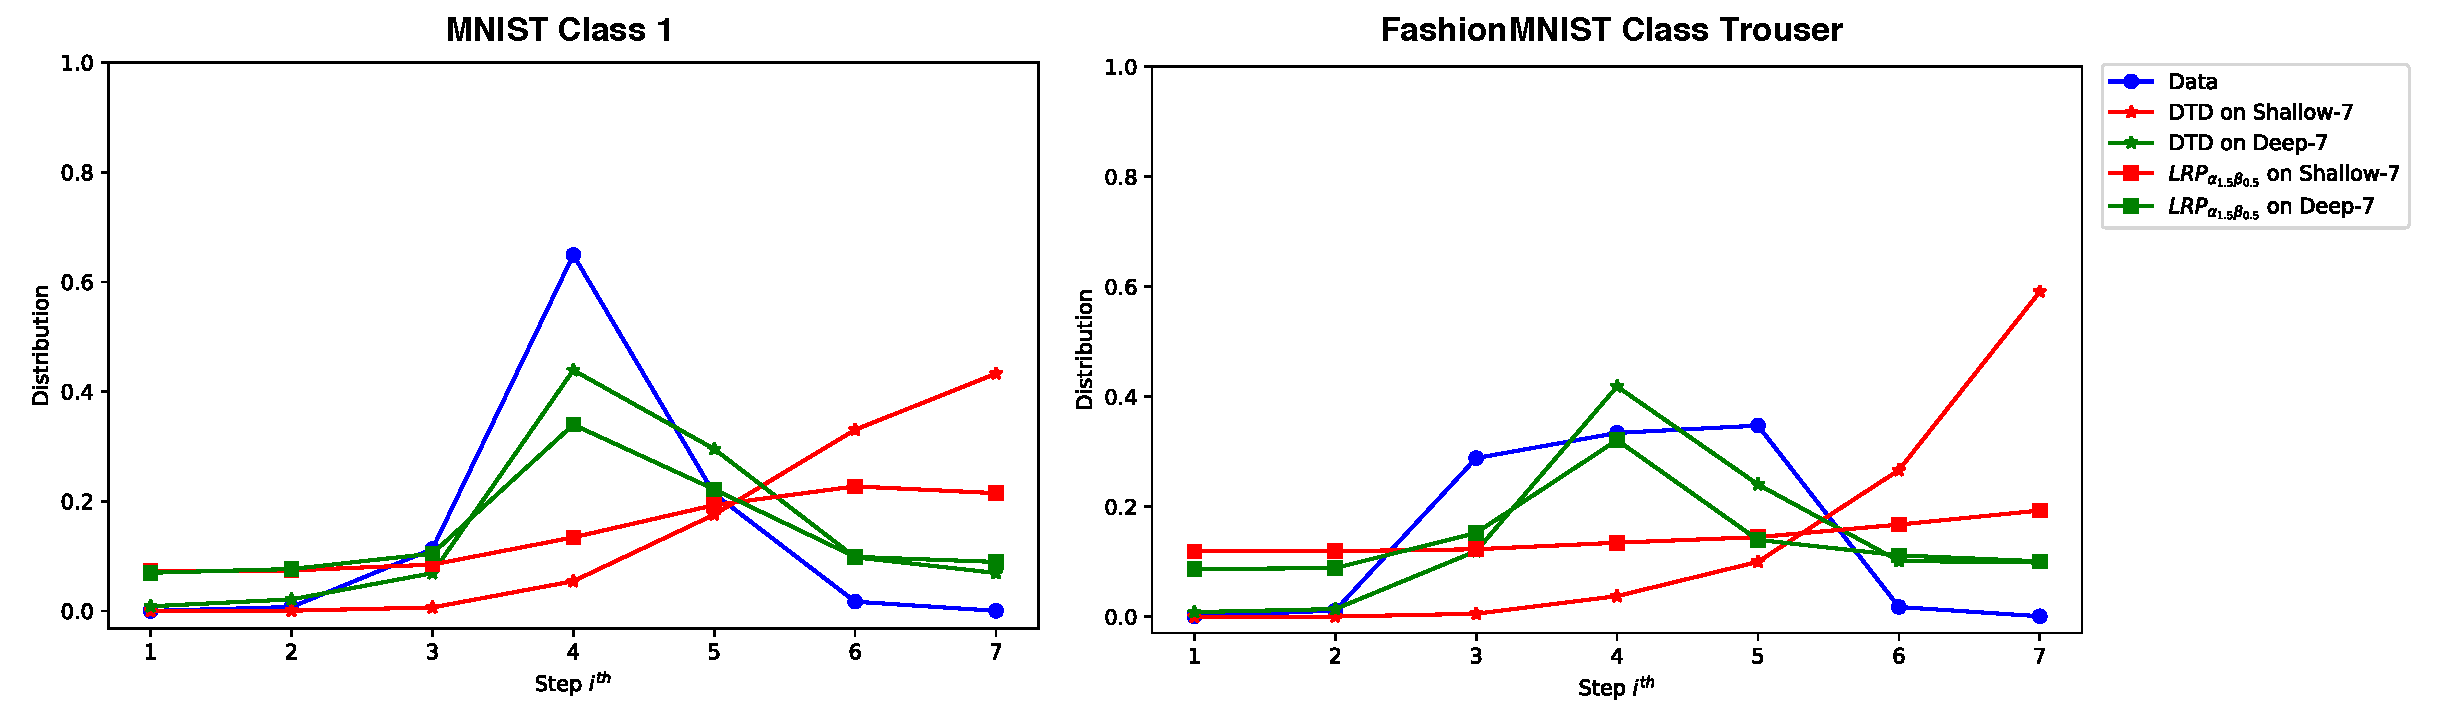
\includegraphics[width=\textwidth]{sketch/exp1_dist_plot}
\caption{Comparison of pixel intensity distribution from MNIST Class 1 testing population and relevance distribution explained by the models} 
\label{fig:exp1_dist_plot}
\end{figure}

%It is worth mentioning that samples in MNIST Class 1 are relatively simples, hence comparing such distributions can give some insight of the explainability of the models. However, in real world setting, qualifying explainability of a neural network via the distributions might not give meaningful intuition, because input tends to have complex structure and the network is likely to produce relevance heatmap that has different structure from the original image. We shall see this behavior in Fashion-MNIST experiments.
%
%
%
%However, one interesting observation I have found is that sensivity analysis ... 


\section{Experiment 2 : Majority Sample Classification}
\subsection{Problem Formulation}

 \begin{figure}[h]
\centering
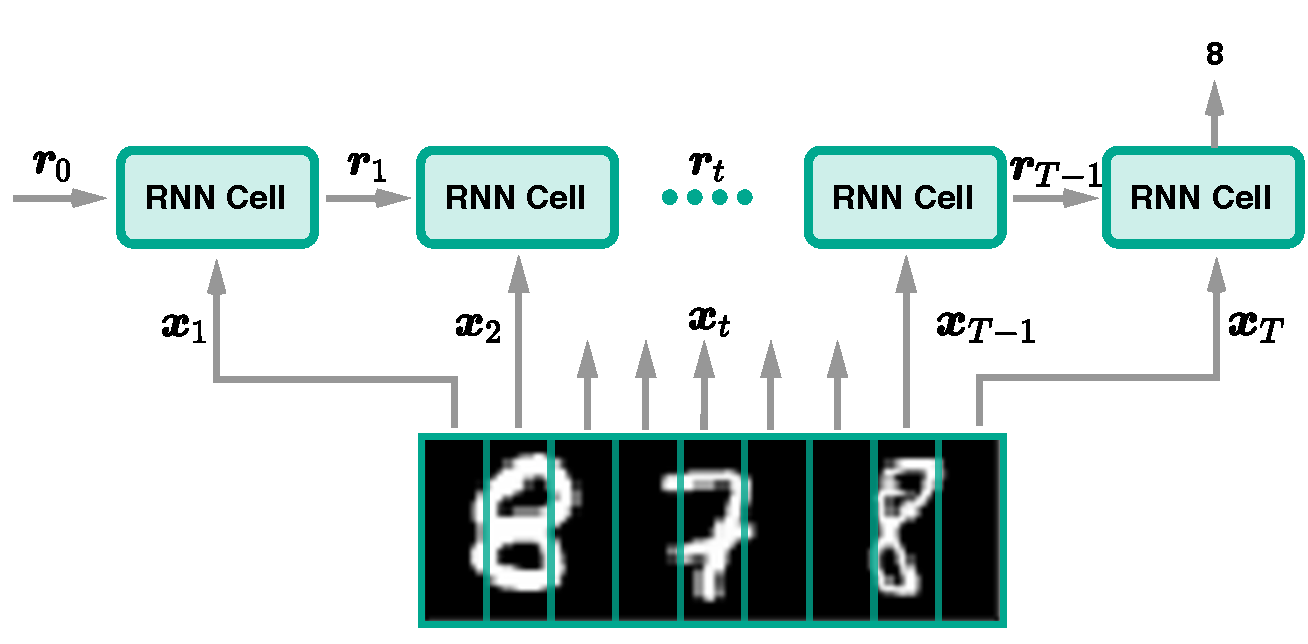
\includegraphics[width=0.7\textwidth]{sketch/artificial_problem_3digits}
\caption{Majority Sample Classification Problem} 
\label{fig:artificial_problem_3digits}
\end{figure}

\subsection{Result}
 \begin{figure}[h]
\centering
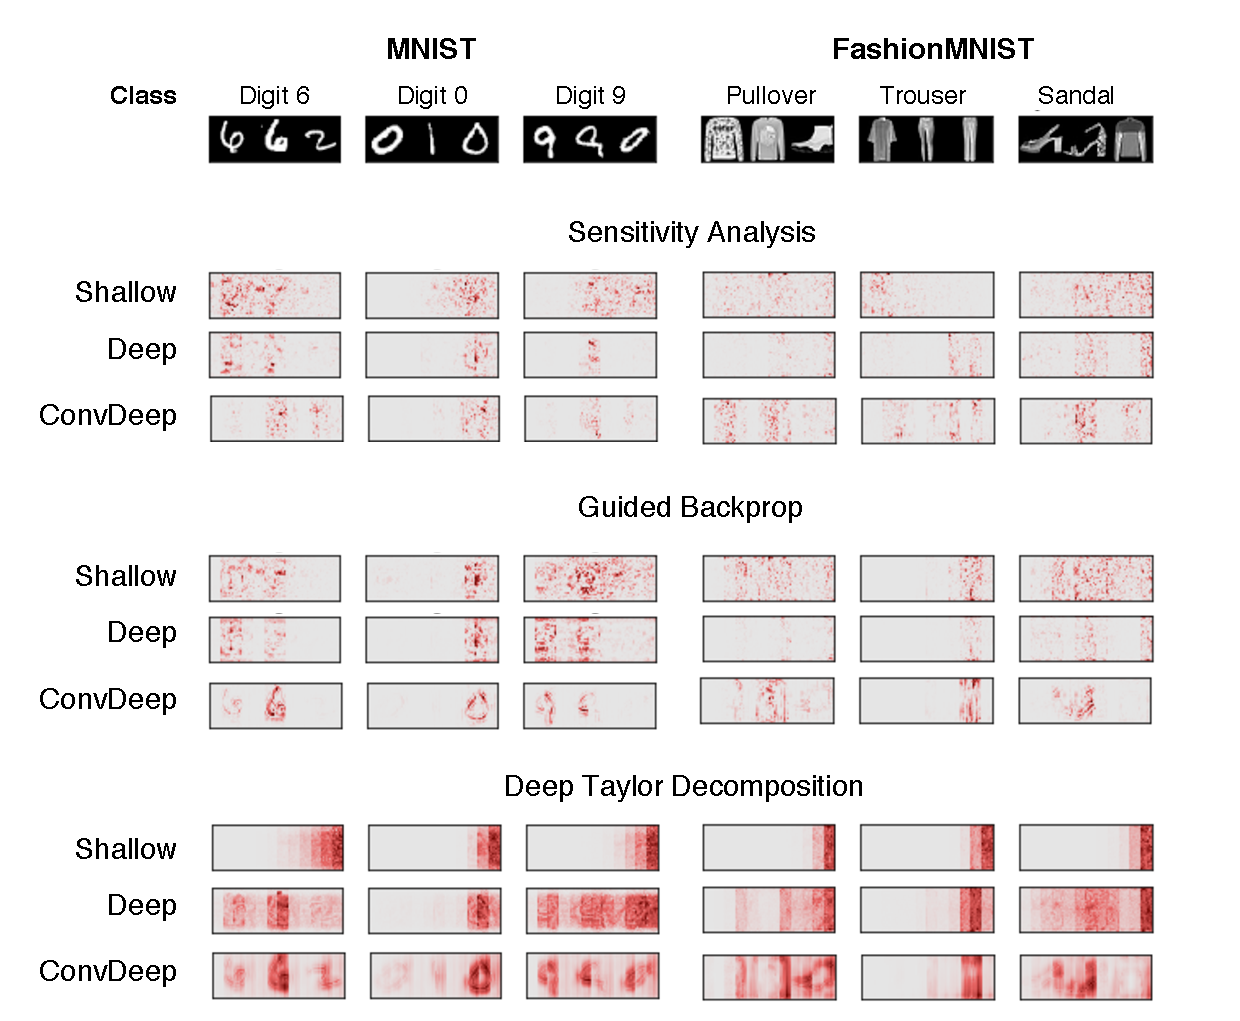
\includegraphics[width=0.7\textwidth]{sketch/heatmap_msc_mix}
\caption{Relevance heamaps for MSC problem} 
\label{fig:heatmap_msc_mix}
\end{figure}

 \begin{figure}[h]
\centering
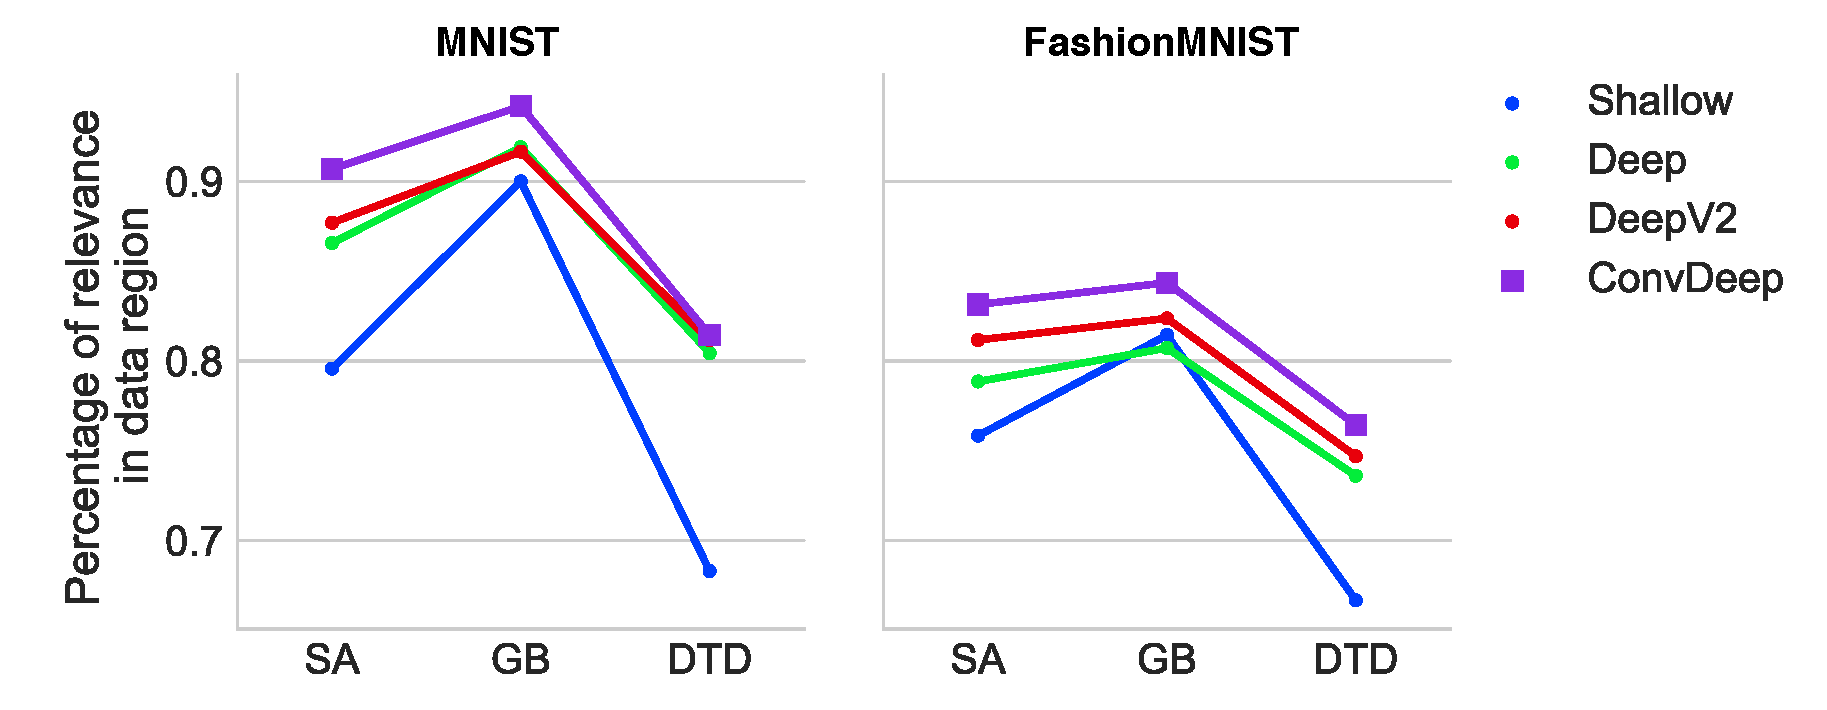
\includegraphics[width=0.7\textwidth]{sketch/rel_dist_maj_3_samples_thesis}
\caption{Percentage of relevance in data region} 
\label{fig:rel_dist_maj_3_samples_thesis}
\end{figure}

\todo{rewrite things from the paper}

\section{Experiment 3 : Improve Relevance Distribution}


%TODO : Add Model accuracy in appendix
